% Options for packages loaded elsewhere
\PassOptionsToPackage{unicode}{hyperref}
\PassOptionsToPackage{hyphens}{url}
\PassOptionsToPackage{dvipsnames,svgnames,x11names}{xcolor}
%
\documentclass[
]{article}
\usepackage{amsmath,amssymb}
\usepackage{lmodern}
\usepackage{setspace}
\usepackage{iftex}
\ifPDFTeX
  \usepackage[T1]{fontenc}
  \usepackage[utf8]{inputenc}
  \usepackage{textcomp} % provide euro and other symbols
\else % if luatex or xetex
  \usepackage{unicode-math}
  \defaultfontfeatures{Scale=MatchLowercase}
  \defaultfontfeatures[\rmfamily]{Ligatures=TeX,Scale=1}
\fi
% Use upquote if available, for straight quotes in verbatim environments
\IfFileExists{upquote.sty}{\usepackage{upquote}}{}
\IfFileExists{microtype.sty}{% use microtype if available
  \usepackage[]{microtype}
  \UseMicrotypeSet[protrusion]{basicmath} % disable protrusion for tt fonts
}{}
\makeatletter
\@ifundefined{KOMAClassName}{% if non-KOMA class
  \IfFileExists{parskip.sty}{%
    \usepackage{parskip}
  }{% else
    \setlength{\parindent}{0pt}
    \setlength{\parskip}{6pt plus 2pt minus 1pt}}
}{% if KOMA class
  \KOMAoptions{parskip=half}}
\makeatother
\usepackage{xcolor}
\IfFileExists{xurl.sty}{\usepackage{xurl}}{} % add URL line breaks if available
\IfFileExists{bookmark.sty}{\usepackage{bookmark}}{\usepackage{hyperref}}
\hypersetup{
  pdftitle={A general model for the evolution of nuptial gift-giving},
  colorlinks=true,
  linkcolor={blue},
  filecolor={Maroon},
  citecolor={Blue},
  urlcolor={Blue},
  pdfcreator={LaTeX via pandoc}}
\urlstyle{same} % disable monospaced font for URLs
\usepackage[margin=1in]{geometry}
\usepackage{graphicx}
\makeatletter
\def\maxwidth{\ifdim\Gin@nat@width>\linewidth\linewidth\else\Gin@nat@width\fi}
\def\maxheight{\ifdim\Gin@nat@height>\textheight\textheight\else\Gin@nat@height\fi}
\makeatother
% Scale images if necessary, so that they will not overflow the page
% margins by default, and it is still possible to overwrite the defaults
% using explicit options in \includegraphics[width, height, ...]{}
\setkeys{Gin}{width=\maxwidth,height=\maxheight,keepaspectratio}
% Set default figure placement to htbp
\makeatletter
\def\fps@figure{htbp}
\makeatother
\setlength{\emergencystretch}{3em} % prevent overfull lines
\providecommand{\tightlist}{%
  \setlength{\itemsep}{0pt}\setlength{\parskip}{0pt}}
\setcounter{secnumdepth}{-\maxdimen} % remove section numbering
\newlength{\cslhangindent}
\setlength{\cslhangindent}{1.5em}
\newlength{\csllabelwidth}
\setlength{\csllabelwidth}{3em}
\newlength{\cslentryspacingunit} % times entry-spacing
\setlength{\cslentryspacingunit}{\parskip}
\newenvironment{CSLReferences}[2] % #1 hanging-ident, #2 entry spacing
 {% don't indent paragraphs
  \setlength{\parindent}{0pt}
  % turn on hanging indent if param 1 is 1
  \ifodd #1
  \let\oldpar\par
  \def\par{\hangindent=\cslhangindent\oldpar}
  \fi
  % set entry spacing
  \setlength{\parskip}{#2\cslentryspacingunit}
 }%
 {}
\usepackage{calc}
\newcommand{\CSLBlock}[1]{#1\hfill\break}
\newcommand{\CSLLeftMargin}[1]{\parbox[t]{\csllabelwidth}{#1}}
\newcommand{\CSLRightInline}[1]{\parbox[t]{\linewidth - \csllabelwidth}{#1}\break}
\newcommand{\CSLIndent}[1]{\hspace{\cslhangindent}#1}
\usepackage{amsmath}
\usepackage{natbib}
\usepackage{lineno}
\usepackage{caption}
\usepackage[utf8]{inputenc}
\bibliographystyle{amnatnat}
\linenumbers
\modulolinenumbers[2]
\ifLuaTeX
  \usepackage{selnolig}  % disable illegal ligatures
\fi

\title{A general model for the evolution of nuptial gift-giving}
\author{Author list (anonymised)}
\date{{[}1{]} Author institutions and email}

\begin{document}
\maketitle

\setstretch{2}
\textbf{Key words:} Nuptial gifts, male search, mate interactions,
modelling, \emph{Pisaura}

\hypertarget{abstract}{%
\section{Abstract}\label{abstract}}

Nuptial gift-giving occurs in several taxonomic groups including
insects, snails, birds, squid, arachnids and humans. Although this trait
has evolved many times independently, no general framework has been
developed to predict the conditions necessary for nuptial gift-giving to
evolve. We use a time-in time-out model to derive analytical results
describing the requirements necessary for selection to favour nuptial
gift-giving. Specifically, selection will favour nuptial gift-giving if
the fitness increase caused by gift-giving exceeds the product of
expected gift search time and encounter rate of the opposite sex.
Selection will favour choosiness in the opposite sex if the value of a
nuptial gift exceeds the inverse of the time taken to produce offspring
multiplied by the rate at which mates with nuptial gifts are
encountered. Selection can differ between the sexes, potentially causing
sexual conflict. We further investigate these results using an
individual-based model inspired by a system of nuptial gift-giving
spiders, \emph{Pisaura mirabilis}, by estimating the fitness benefit of
nuptial gift-giving using experimental data from several studies. Our
results provide a general framework for understanding when the evolution
of nuptial gift-giving can occur and provide novel insight into the
evolution of worthless nuptial gifts, occurring in multiple taxonomic
groups with implications for understanding parental investment.

\hypertarget{introduction}{%
\section{Introduction}\label{introduction}}

Nuptial gift-giving occurs when the choosy sex (usually the female)
receives gifts from the opposite sex (usually the male) during
courtship. It is a widespread phenomenon, occurring within several
diverse taxonomic groups such as insects, snails, birds, squid,
arachnids and humans (\protect\hyperlink{ref-Lewis2012}{Lewis \& South,
2012}; \protect\hyperlink{ref-Albo2014}{Albo \emph{et al.}, 2014};
\protect\hyperlink{ref-Lewis2014}{Lewis \emph{et al.}, 2014}). Despite
the ubiquity of this behaviour, little effort has been made to
conceptualise the evolution of nuptial gift-giving within a general
modelling framework (\protect\hyperlink{ref-Lewis2014}{Lewis \emph{et
al.}, 2014}; \protect\hyperlink{ref-Iwasa2022}{Iwasa \& Yamaguchi,
2022}). Recent models describing the evolution of nuptial gift-giving
have focused on co-evolution between male nuptial gift-giving and female
propensity to remate, and evolutionarily stable nuptial gift sizes
(\protect\hyperlink{ref-Kamimura2021}{Kamimura \emph{et al.}, 2021};
\protect\hyperlink{ref-Iwasa2022}{Iwasa \& Yamaguchi, 2022}), but a
general framework describing the conditions under which nuptial
gift-giving can be initially favoured by selection is needed to
understand when gift-giving should evolve.

Nuptial gift-giving may allow males to increase fitness by acquiring
additional mates, indirect benefits (by increasing offspring fitness),
prolonged copulations, and success in sperm competition
(\protect\hyperlink{ref-Albo2013}{Albo \emph{et al.}, 2013};
\protect\hyperlink{ref-Ghislandi2014}{Ghislandi \emph{et al.}, 2014};
\protect\hyperlink{ref-Lewis2014}{Lewis \emph{et al.}, 2014}). However,
this potential fitness increase comes at the expense of producing a
nuptial gift, which may be costly in terms of time and resources.
Females may increase their fitness by receiving nutritionally valuable
nuptial gifts, but expressing a preference for males with gifts might
result in a mating opportunity cost if available males without gifts are
rejected. With respect to nuptial gift-giving, the evolutionary
interests of both sexes may not always fully overlap. This can cause
sexual conflict, which is a difference in the fitness interests between
sexes that occurs when an interaction results in a situation where
individuals cannot both achieve an optimal outcome
(\protect\hyperlink{ref-Parker2006}{Parker, 2006}). For example, under
some conditions, it might be optimal for males to mate without offering
a nuptial gift, while it might be optimal for females to insist on
receiving a nuptial gift.

Much work has sought to explain how gift-giving tactics are maintained,
with explanations including condition-dependent strategies, gift-giving
as a way to decrease female aggression during copulation, or gifts as
sensory traps (\protect\hyperlink{ref-Lubin2007}{Lubin \& Bilde, 2007};
\protect\hyperlink{ref-Toft2016}{Toft \& Albo, 2016};
\protect\hyperlink{ref-Ghislandi2018}{Ghislandi \emph{et al.}, 2018};
\protect\hyperlink{ref-Albo2019}{Albo \emph{et al.}, 2019}). An example
of such a system is the nuptial gift-giving nursery-web spider
\emph{Pisaura mirabilis}, where males may court females with or without
nuptial gifts (\protect\hyperlink{ref-Bristowe1926}{Bristowe \& Locket,
1926}; \protect\hyperlink{ref-Tuni2013a}{Tuni \emph{et al.}, 2013}).
Here, males may provide females with costly nuptial gifts in the form of
captured arthropod prey, and females may exhibit preference for males
with a nuptial gift by rejecting males without a nuptial gift
(\protect\hyperlink{ref-Albo2013}{Albo \emph{et al.}, 2013}).

We develop a general framework for investigating the evolution of
nuptial gift-giving and choosiness using a time-in, time-out modelling
approach and an individual-based model
(\protect\hyperlink{ref-Clutton-Brock1992}{Clutton-Brock \& Parker,
1992}). Specifically, we derive conditions under which selection will
favour male search for nuptial gifts and female rejection of gift-less
males. We show that selection for searching and choosiness depends on
whether a threshold fitness value of the nuptial gift is exceeded. Our
model demonstrates the importance of nuptial gift cost, sex ratio, and
mate encounter rate in determining the threshold above which selection
will favour the evolution of nuptial gift-giving. Importantly, we show
that the threshold value differs for male searching and female
choosiness. We complement the predictions of our analytical model by
formulating an individual-based model, which further supports the main
theoretical results. We apply our model to an example system with
nuptial gifts, the nursery web spider \emph{Pisaura mirabilis}, where we
use experimental data to estimate a key model parameter. Our results
provide a general framework for understanding why nuptial gift-giving
evolves in some systems and not in others, how the evolution of nuptial
gift-giving can give rise to sexual conflict, and it provides insight
into the evolution of worthless and deceitful nuptial gifts, which occur
in several different taxonomic (\protect\hyperlink{ref-LeBas2005}{LeBas
\& Hockham, 2005}; \protect\hyperlink{ref-Ghislandi2014}{Ghislandi
\emph{et al.}, 2014}).

\hypertarget{model}{%
\section{Model}\label{model}}

We use a time-in and time-out model
(\protect\hyperlink{ref-Clutton-Brock1992}{Clutton-Brock \& Parker,
1992}; \protect\hyperlink{ref-Kokko2001}{Kokko \& Monaghan, 2001};
\protect\hyperlink{ref-Kokko2006}{Kokko \& Ots, 2006}) in which choosy
(female) and non-choosy (male) individuals spend some period of time
within the mating pool searching for a mate (time-in) followed by a
period outside the mating pool (time-out). During time-out, females
spend some duration of time (\(T_{\mathrm{f}}\)) gestating or rearing
(hereafter `processing') offspring. We define the number of offspring
produced by a female per reproductive cycle as \(\lambda\). Since
females enter time-out after mating, this is equivalent to assuming a
system with sequential polyandry. For simplicity, we assume male time to
replenish sperm is negligible, but males can spend some duration of time
out of the mating pool searching for nuptial gifts. We define
\(T_{\mathrm{m}}\) as the time until a gift is found by a searching
male.

\begin{figure}
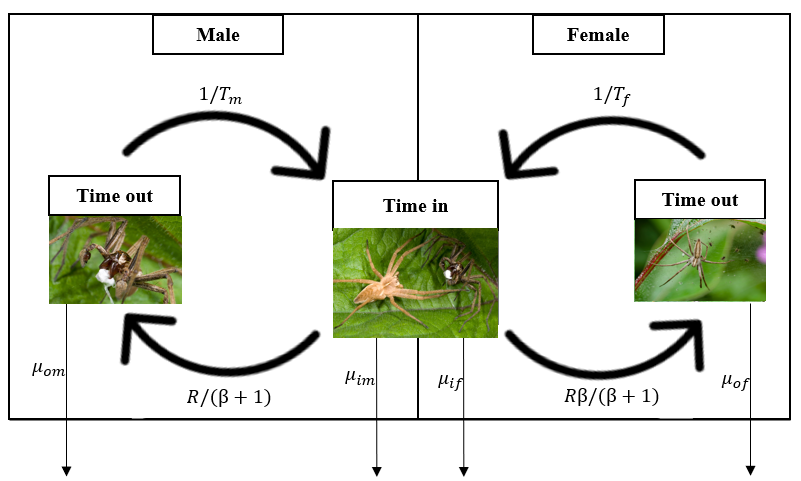
\includegraphics[width=1\linewidth]{inst/img/conceptual_figure} \caption{Conceptual figure inspired by Kokko and Ots (2006) illustrating how the modelling framework maps onto an example of a system wherein nuptial gifts are used, here \textit{Pisaura mirabilis}. Males have a probability of obtaining a nuptial gift while in time-out, which will affect their probability of mating while in time-in. They return to the mating pool (time-in) at a rate determined by the time spent searching for a nuptial gifts ($T_{\mathrm{m}}$) and leave the mating pool (i.e. enter time-out) following the female encounter rate, which is dependent on the ratio of males to females ($\beta$) and the encounter rate ($R$). The choosy sex (females) enter the mating pool at a rate depending on the time spent processing offspring ($T_{\mathrm{f}}$) and leave the mating pool (i.e. enter time-out) at a rate that is dependent on $\beta$ and $R$. Males and females undergo sex-specific mortality $\mu$ during time-in and time-out. Image left to right: (1) male \textit{P. mirabilis}. (2) male \textit{P. mirabilis} presenting nuptial gift (white) to female. (3) Female \textit{P. mirabilis} protecting offspring. Photos: Alamy.}\label{fig:unnamed-chunk-2}
\end{figure}

\hypertarget{analytical-model}{%
\subsection{Analytical model}\label{analytical-model}}

The probability that a male succeeds in securing a nuptial gift (\(G\))
after a duration of \(T_{\mathrm{m}}\) is defined by,

\[P(G) = 1 - e^{-\frac{1}{\alpha}T_{m}}.
\tag{1}
\]

In Eq. 1, \(\alpha\) defines expected search time before encountering a
nuptial gift. Thus, the probability of finding a nuptial gift is higher
the more time is spent searching. During time-in, individuals encounter
conspecifics at a rate of \(R\). A focal individual will therefore
encounter conspecifics of the opposite sex at a rate of \(R/2\) if the
ratio of males to females in the mating pool (\(\beta\)) is equal. More
generally, males will be encountered at a rate of \(R\beta/(\beta+1)\),
and females will be encountered at a rate of \(R/(\beta+1)\). An example
of how the structure of the time-in time-out model applies to a system
with nuptial gift-giving is given in Figure 1. We assume that mating
with a nuptial gift increases expected offspring production by an
increment of \(\gamma\). Mortality occurs for females and males in
(\(\mu_{\mathrm{i,f}}\), \(\mu_{\mathrm{i,m}}\)) and out
(\(\mu_{\mathrm{o,f}}\), \(\mu_{\mathrm{o,m}}\)) of the mating pool.
Following Kokko \& Ots (\protect\hyperlink{ref-Kokko2006}{2006}), we
assume \(m_{\mathrm{i,f}} = m_{\mathrm{o,f}} = 1\) and
\(m_{\mathrm{i,m}} = m_{\mathrm{o,m}} = 1\).

First, we find the fitness of males that search versus do not search for
a nuptial gift. We then describe the fitness consequences of female
choice to accept or reject males based on their provision of a nuptial
gift. We can then calculate the thresholds \(\gamma_{\mathrm{m}}\) and
\(\gamma_{\mathrm{f}}\) above which males and females are favoured by
selection to search for nuptial gifts and exhibit choosiness for nuptial
gifts, respectively.

\emph{Male fitness}

During time-out, males can search for a nuptial gift. Males can adopt
one of two strategies; either search or do not search for a nuptial
gift. Males with the searching strategy continue to search until they
find a nuptial gift, while males that do not search immediately re-enter
the mating pool. Consequently, time searching for a nuptial gift will
come at the cost of mating opportunities but might increase offspring
fitness. We therefore need to model the expected length of time spent
outside of the mating pool for males that search for nuptial gifts
(\(E[T_{\mathrm{m}}]\)), which equals \(\alpha\). We can integrate
search time \(t\) over the rate at which nuptial gifts are encountered
(\(\exp(-1/\alpha)\)) to show \(E[T_{\mathrm{m}}] = \alpha\),

\[E[T_{\mathrm{m}}] = \int_{0}^{\infty}e^{- \frac{1}{\alpha}t}dt = \alpha.\]

The rate at which a focal male that searches for a nuptial gift
increases his fitness is therefore his reproductive output
\(\lambda(1 + \gamma)\) divided by expected time spent searching for a
nuptial gift (\(\alpha\)) plus time spent in the mating pool,
\((\beta + 1)/R\),

\[W_{\mathrm{M_{G}}} = \lambda \frac{1 + \gamma}{\alpha + \left( \frac{\beta + 1}{R} \right)}.\]

In contrast, a male that does not search for a nuptial gift has fewer
offspring, but spends less time outside of the mating pool,

\[W_{\mathrm{M_{L}}} = \lambda \frac{1}{\left(\frac{\beta+1}{R} \right)} = \lambda \frac{R}{\beta + 1}.\]

We can determine the conditions for which
\(W_{\mathrm{M_{G}}} > W_{\mathrm{M_{L}}}\), isolating \(\gamma\) to
find how large of a fitness benefit must be provided by the nuptial gift
to make the search cost worthwhile, which simplifies to,

\[\gamma_{\mathrm{m}} > \alpha \frac{R}{\beta + 1}.
\tag{2}
\]

When this inequality holds, males are favoured to search until they find
a nuptial gift, which would result in an average search time of
\(\alpha\). If the male trait is instead continuous (i.e., males search
for time period \(T_{\mathrm{m}}\)), it can be shown that the same
threshold can be reached by evaluating the partial derivative of the
male fitness function (Supporting Information S1). Hence, the thresholds
are consistent under different assumptions concerning male searching
strategy. Selection will cause males to search for nuptial gifts if the
fitness increase to offspring exceeds the product of search time and
female encounter rate.

\emph{Female fitness}

During time-out, females process offspring over a duration of
\(T_{\mathrm{f}}\) (we assume that \(T_{\mathrm{f}} > \alpha\),
otherwise females are not the choosy sex). When females re-enter the
mating pool, they encounter males at a rate of \(R\beta/(\beta + 1)\).
If a female encounters a male with a nuptial gift, we assume that she
will mate with him. But if a female encounters a male with no nuptial
gift, then she might accept or reject the male. If she rejects the male,
then she will remain in the mating pool. The rate at which a female
encounters a male with a nuptial gift is,

\[R_{\mathrm{F_{G}}} = R \left(\frac{\beta}{\beta + 1}\right)\left(1 - e^{-\frac{1}{\alpha}T_{\mathrm{m}}}\right).\]

Expected time spent in the mating pool before a focal female encounters
a male with a gift will be \(1/R_{\mathrm{F_{G}}}\). The rate at which a
female increases her fitness by being choosy and mating only when she
encounters a male with a gift is,

\[W_{f, g} = \lambda \frac{1 + \gamma}{T_{F} + \frac{1}{R_{\mathrm{F,G}}}}.
\tag{4}
\]

The top of the right-hand side of Eq. 4 gives her fitness increase, and
the bottom gives the total time it takes to obtain this fitness. The
\(R_{\mathrm{F_{G}}}\) is inverted because it represents the expected
time to encountering a male with a gift. We can expand Eq. 6,

\[W_{\mathrm{F_{G}}} = \lambda \frac{1 + \gamma}{T_{\mathrm{f}} + \frac{1}{R \left(\frac{\beta}{\beta + 1}\right)\left(1 - e^{-\frac{1}{\alpha}T_{\mathrm{m}}}\right)}}.\]

If the focal female is not choosy and accepts the first male that she
encounters, then the rate at which she increases her fitness is,

\[W_{\mathrm{F_{G,L}}} = \lambda \frac{\left(1 + \gamma\right)\left(1 - e^{-\frac{1}{\alpha}T_{\mathrm{m}}}\right) + e^{-\frac{1}{\alpha}T_{\mathrm{m}}}}{T_{f} + \frac{1}{R \left(\frac{\beta}{\beta + 1}\right)}}.\]

We then evaluate the conditions under which
\(W_{\mathrm{F_{G}}} > W_{\mathrm{F_{G,L}}}\). We can isolate \(\gamma\)
to determine how much offspring fitness must be increased to make
choosiness beneficial (\(\gamma_{\mathrm{f}}\)),

\[\gamma_{\mathrm{f}} > \frac{1}{T_{\mathrm{f}} R\left(\frac{\beta}{\beta + 1}\right) \left(1 - e^{-\frac{1}{\alpha}T_{\mathrm{m}}}\right)}.
\tag{5}
\]

Note that that the expression
\(R\left(\frac{\beta}{\beta + 1}\right) \left(1 - e^{-1\frac{1}{\alpha}T_{\mathrm{m}}}\right)\)
defines the rate at which a female in the mating pool encounters males
with nuptial gifts. Hence, female choosiness is ultimately determined by
time spent out of the mating pool to process offspring
(\(T_{\mathrm{f}}\)) and the rate at which a female in the mating pool
encounters males with nuptial gifts.

\emph{Operational sex ratio}

We assume that the sex ratio is equal upon maturation. Given this, Kokko
\& Monaghan (\protect\hyperlink{ref-Kokko2001}{2001}) show that the
operational sex ratio depends on the probability of finding an
individual in time-in,

\[\beta = \frac{\int_{t = 0}^{\infty} P_{IM}(t)dt}{\int_{t = 0}^{\infty} P_{IF}(t)dt}.
\tag{6}
\]

In Eq. 6, \(P_{IM}(t)\) and \(P_{IF}(t)\) are the probabilities of
finding a male and female in time-in, respectively. There is no closed
form solution to the operational sex ratio, so we used recursion to
calculate \(\beta\) values for a given \(T_{\mathrm{f}}\),
\(T_{\mathrm{m}}\), and \(R\) (see Supporting Information S2),

\hypertarget{individual-based-model}{%
\subsection{Individual-based model}\label{individual-based-model}}

We formulate an individual-based time-in time-out simulation model to
complement the predictions made by our analytical time-in time-out model
above and further allow for coevolution between male search behaviour
and female choosiness. Here we describe the details of initialisation,
time-in (mating), time-out (reproduction and nuptial gift search), and
mortality. We then summarise the simulations run and data collected.

\emph{Initialisation}

Before the first time step, a population of \(N = 1000\) individuals is
initialised. Individuals are assigned to be female with a probability of
\(0.5\), else male. Female offspring processing time for a focal
individual \(i\) is fixed at \(T^{i}_{\mathrm{f}} = 2\). Each individual
is initialised with a diploid genotype that underlies female rejection
probability of gift-less males (\(\rho^{i}\)), and a diploid genotype
that underlies male search time (\(T^{i}_{\mathrm{m}}\)). Alleles can
take any real value and combine additively to determine \(\rho^{i}\) and
\(T^{i}_{\mathrm{m}}\). For all simulations, initialised values are set
to , \(\rho^{i} = 0\), and \(T^{i}_{\mathrm{m}} = 0\). All individuals
are initialised outside of the mating pool in the first time step
\(t = 1\). The first time step then proceeds with females immediately
entering the mating pool and males either entering the mating pool or
searching for nuptial gifts.

\emph{Time-in}

At the start of each time step, females and males in the mating pool
remain in it. Females outside the mating pool enter the mating pool
after processing offspring, and males enter it after searching for
nuptial gifts (see `Time-out' below). Up to \(\Psi = N\psi\)
interactions between individuals can occur in a single time step, where
\(\psi\) is a scaling parameter. In each time step, \(\Psi\) pairs of
individuals are selected at random to interact. For each interaction,
two different individuals are randomly selected from the population with
equal probability. If the selected individuals are of different sexes,
and both are in the mating pool, then a mating encounter occurs. If the
male does not have a nuptial gift, then a focal female \(i\) will reject
him with a probability of \(\rho^{i}\); if rejection occurs, then both
individuals stay in the mating pool. If rejection does not occur, or the
male has a nuptial gift in the mating encounter, then the individuals
mate. Females then leave the mating pool and enter time-out to process
offspring, and males leave and enter time-out to potentially search for
new nuptial gifts (note that females and males might re-enter the mating
pool immediately within the same time step given sufficiently low search
time; see Time-out below).

\emph{Time-out}

During time-out, offspring production and time outside of the mating
pool are realised for each female by sampling from a Poisson
distribution. A focal female \(i\) will produce
\(\mathrm{Poisson}(\lambda)\) offspring if no nuptial gift was provided
or \(\mathrm{Poisson}(\lambda + \gamma)\) if a gift was provided.
Females remain outside of the mating pool to process offspring for
\(\mathrm{Poisson}(T^{i}_{\mathrm{f}})\) time steps. Offspring are added
to the population immediately, with one \(\rho^{i}\) and one
\(T^{i}_{\mathrm{m}}\) allele sampled from each parent with complete
recombination. Mutation occurs independently for each allele with a
probability of \(\epsilon = 0.001\), and if mutation occurs, then a new
allele value is sampled from a normal distribution mean centred on the
existing value with a standard deviation of \(\sigma_{\epsilon} = 0.1\).
Offspring sex is randomly assigned with equal probability as female or
male. Female offspring are immediately placed in the mating pool, and
male offspring are out of the mating pool to potentially search for
nuptial gifts. After a female has spent
\(\mathrm{Poisson}(T^{i}_{\mathrm{f}})\) time steps outside the mating
pool, she will re-enter it.

A focal male \(i\) outside the mating pool will enter it if he has
searched for a fixed number of \(T^{i}_{\mathrm{m}}\) time steps, which
is also sampled randomly from a Poisson distribution,
\(\mathrm{Poisson}(T^{i}_{\mathrm{m}})\). If \(T^{i}_{\mathrm{m}} = 0\),
then the male immediately returns to the mating pool (in the same time
step). If \(T^{i}_{\mathrm{m}} > 0\), then the male must wait outside
the mating pool for \(\mathrm{Poisson}(T^{i}_{\mathrm{m}})\) time steps,
but will enter the mating pool with a nuptial gift with a probability,

\[P(G^{i}) = 1 - e^{-\frac{1}{\alpha}T^{i}_{\mathrm{m}}}.\]

Males must always spend \(\mathrm{Poisson}(T^{i}_{\mathrm{m}})\) time
steps outside of the mating pool regardless of whether or not they are
successful in obtaining a nuptial gift.

\emph{Mortality}

At the end of each time step, mortality occurs first with a fixed
probability for all adults in the population, then with a probability
caused by carrying capacity \(K = 1000\) applied to all individuals
(adults and offspring). Mortality occurs in each time step with a fixed
probability of \(\mu\) regardless of the sex of the individual or its
position in or out of the mating pool. If after this fixed mortality is
applied, the total population size \(N > K\), then individuals are
removed at random with equal probability until \(N = K\). Following
adult mortality, a new time step begins with newly added offspring
becoming adults.

\emph{Simulations}

We ran simulations in which male search time and female choosiness
evolved from an ancestral state of no searching and no choosiness. In
all simulations, \(N\) was initialised at 1000 and \(K = 1000\).
Simulations ran for \(t_{max} = 10000\) time steps. We set
\(T_{\mathrm{f}} = 2\), \(\psi = 3\), and \(\lambda = 1\) for all
simulations, and we simulated across a range of
\(\alpha = \{0.1, 0.2, ..., 1.9, 2.0\}\) and
\(\gamma = \{0, 0.1, ..., 1.9, 2.0\}\) parameter values for 5000
replicates. In a sensitivity analysis, we also re-ran simulations for
values of \(T_{\mathrm{f}} = 10\) and \(\psi = \{1, 2, 4, 6 \}\) (see
Supporting Information S3), and simulated the evolution of male nuptial
gift searching and female choosiness (fixing
\(T_{\mathrm{m}} = \alpha\)) separately (see Supporting Information S4).
Summary statistics for mean trait values, population size, sex ratios,
proportion of females and males in and out of the mating pool, and mean
number of encounters per female and male within the mating pool were all
calculated in the last time step. The C code used for simulating these
IBMs also allows for the reporting of summary statistics in each time
step. Additionally, it can simulate explicit space and individual
movement through the landscape. A neutral evolving trait was also
modelled to ensure that the code functioned as intended, and processes
were compartmentalised into individual functions to facilitate code
testing. All code is publicly available on GitHub
(\url{https://github.com/AUTHOR_NAME/REPOSITORY_NAME}).

\emph{Application to gift-giving spiders}

We can produce an estimate of the fitness increment obtained by females
when receiving a gift (\(\hat{\gamma}\)) by using data on female
\emph{P. mirabilis} egg production and hatching success
(\protect\hyperlink{ref-Tuni2013a}{Tuni \emph{et al.}, 2013}). Tuni
\emph{et al.} (\protect\hyperlink{ref-Tuni2013a}{2013}) found
differences in egg production and hatching success in female \emph{P.
mirabilis} under different feeding regimes. Assuming these differences
in feeding regimes correspond to eating versus not eating nuptial gifts,
the mean number of offspring produced by a female who eats nuptial gifts
can be calculated. This calculation will be an overestimate because
females that were fed in Tuni \emph{et al.}
(\protect\hyperlink{ref-Tuni2013a}{2013}) received multiple nuptial
gifts. Nevertheless, we calculate these means using raw data from Tuni
\emph{et al.} (\protect\hyperlink{ref-Tuni2013a}{2013}) and find that
mean offspring produced by females receiving nuptial gifts is
\(25.74 \pm 0.96\), while offspring produced by females without a
nuptial gift is \(6.00 \pm 2.1\). Consequently, the relative gain in
fitness from receiving a nuptial gift for a female is estimated to be
\(\hat{\delta_\mathrm{f}} = 25.74 / 6.00 = 4.29\). Since the baseline
fitness is 1, the increase in fitness resulting from a nuptial gift then
becomes \(\hat{\gamma} = \hat{\delta_{\mathrm{f}}} - 1 = 3.29.\)

\hypertarget{results}{%
\section{Results}\label{results}}

Our model predicts 4 zones that are delineated by inequalities 2 and 5
and describe the initial thresholds for the evolution of searching for
nuptial gifts in males and choosiness for nuptial gifts in females.
Figure 2a illustrates conditions under which no searching or choosiness
evolves (zone A), only search (zone B) or choosiness (zone C) evolve, or
both searching and choosiness evolve (zone D). Blue and red threshold
lines in Figure 2 are defined by Eq. 2 and Eq. 5, respectively. Figure
2b illustrates the expansion of zone B as encounter rate decreases,
which is consistent with the results of our IBM (Figure 3).

\begin{figure}
\centering
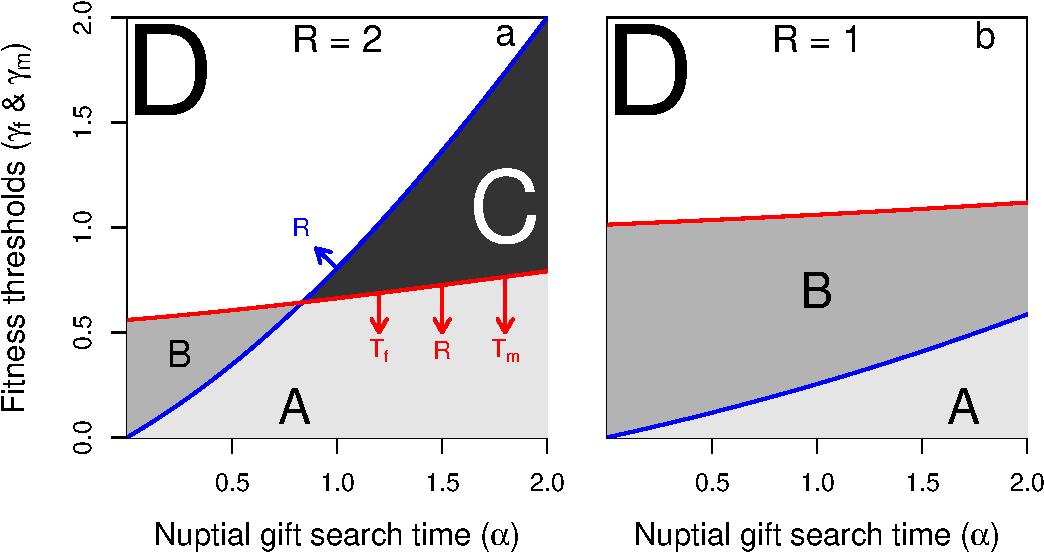
\includegraphics{ms_files/figure-latex/unnamed-chunk-3-1.pdf}
\caption{Fitness thresholds above which males increase their fitness by
searching for nuptial gifts (blue lines; Eq. 2) and females increase
their fitness by rejecting males that do not offer gifts (red lines; Eq.
3). Parameter space includes areas in which males do not search for
nuptial gifts and females are not choosy (A), males search but females
are not choosy (B), females would be choosy but males do not search (C),
and males search and females are choosy (D). Arrows in panel a indicate
the effect of increasing encounter rate (\(R\)), female time-out
(\(T_{\mathrm{f}}\)), and male search time (\(T_{\mathrm{m}}\)). As an
example, trajectories for \(T_{\mathrm{f}} = 2\), and
\(T_{\mathrm{m}} = \alpha\) are shown for values of \(R=2\) (panel a)
and \(R = 1\) (panel b). Females are assumed to be the choosy sex, which
is maintained as long as \(\alpha < T_{\mathrm{f}}\).}
\end{figure}

For males, if nuptial gifts are not abundant and thus require a long
time to find (i.e., high \(\alpha\)), or if males encounter many females
per unit time (i.e., high \(R / (1+\beta)\)), then the nuptial gift must
result in a high fitness increment for selection to favour searching.
For females, if \(\gamma\) is sufficiently high, fitness is increased by
rejecting males without gifts and mating only with males that provide
nuptial gifts. As offspring processing time (\(T_{\mathrm{f}}\)), mate
encounter rate (\(R\beta / (\beta + 1)\)), or the probability of a male
finding a nuptial gift (\(1 - \exp(-T_{\mathrm{m}}/\alpha)\) ) decrease,
the threshold value of fitness above which selection will favour
choosiness (\(\gamma_{\mathrm{f}}\)) increases. This can be understood
intuitively by realising that rejecting a prospective male represents an
opportunity cost for the female.

\begin{figure}
\centering
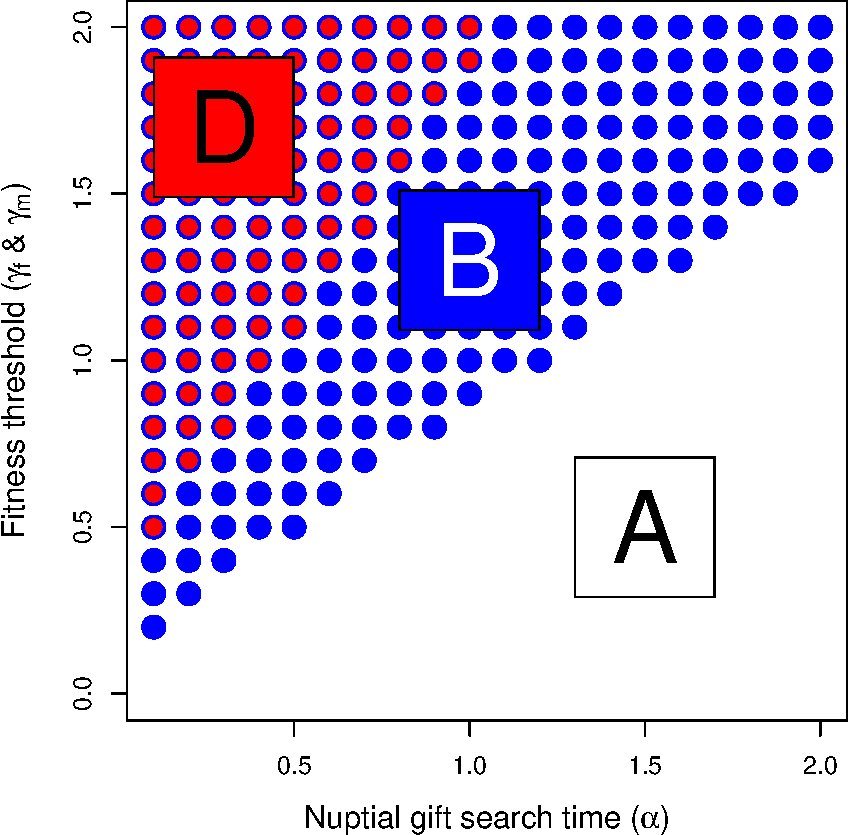
\includegraphics{ms_files/figure-latex/unnamed-chunk-4-1.pdf}
\caption{The coevolution of male search and female choosiness as a
function of nuptial gift search time (\(\alpha\)). Points show where the
lower 95\% confidence interval of female choosiness (red) and male
search (blue) exceeds zero, indicating evolution of choosiness or
nuptial gift search. Each point includes data from 5000 replicate
simulations with identical starting conditions. Zones are identified
that correspond to areas where males search and females are choosy (D),
males search but females are not choosy (B), and males do not search and
females are not choosy (A), as also depicted in Figure 2. The number of
individuals in the population remained at or near carrying capacity of
\(K = 1000\). In each time step, up to 3000 total pair-wise interactions
occurred. Expected female processing time was set to
\(T_{\mathrm{f}}=2\) time steps, and \(\gamma\) and \(\alpha\) values in
the range {[}0.0, 2.0{]} and {[}0.1, 2.0{]}, respectively, were used.}
\end{figure}

Individual-based model results recover zones A, B, and D (Figure 3). In
other words, IBM simulations demonstrate that nuptial gift search in
males, and choosiness in females, will evolve from an ancestral state of
no searching and no choosiness in similar parameter space (Figure 3) as
predicted by the analytical model (Figure 2b). Further, although it was
not possible to parameterise our model for the \emph{P. mirabilis}
system in detail, our calculated value of \(\hat{\gamma} = 3.29\) is
consistent with the evolution of nuptial gift searching and choosiness
recovered by our analytical model and IBM.

\hypertarget{discussion}{%
\section{Discussion}\label{discussion}}

Nuptial gift-giving has arisen several times independently throughout
the animal kingdom (\protect\hyperlink{ref-Lewis2012}{Lewis \& South,
2012}), so understanding how selection favours nuptial gift giving and
choosiness is important for a broad range of mating systems. We provide
a general framework that defines the necessary conditions for selection
to favour the evolution of nuptial gift-giving. We show that males
should give nuptial gifts if the value of a nuptial gift exceeds a
threshold dependent on the encounter rate between females and males and
the cost or time necessary to find or produce a nuptial gift. This
result makes intuitive sense because if males rarely encounter females,
time searching for a gift is a minor cost relative to mate search time.
If males encounter many females, it is not worth seeking nuptial gifts
unless gifts are very valuable since the male will meet many prospective
mates, and nuptial gift search time might come at a cost of decreased
mating opportunities. In practice, male biased sex ratios will not
necessarily favour male search for nuptial gifts if the female encounter
rate is very high, so the key variable is how often males and females
encounter each other. If the search time or cost of finding a nuptial
gift is high, nuptial gifts must be very valuable before search is
favoured by selection. We also show that females should express
choosiness for males with nuptial gifts if the value of the nuptial gift
exceeds the inverse of the product of offspring processing time and
encounter rate with males holding gifts.

\hypertarget{threshold-fitness-values}{%
\subsection{Threshold fitness values}\label{threshold-fitness-values}}

We show that the threshold nuptial gift value at which females are
favoured to express choosiness for nuptial gifts is rarely equivalent to
the threshold value at which males are favoured to search for nuptial
gifts, potentially leading to sexual conflict
(\protect\hyperlink{ref-Arnqvist2005a}{Arnqvist \& Rowe, 2005};
\protect\hyperlink{ref-Oliveira2008}{Oliveira \emph{et al.}, 2008}).
Here, we are defining sexual conflict as occurring when interactions
between sexes result in situation where both sexes cannot achieve an
optimal outcome simultaneously
(\protect\hyperlink{ref-Parker2006}{Parker, 2006}). As an example,
sizable areas of parameter space exists wherein the female optimum would
be to exhibit preference for (and receive) nuptial gifts, while the male
optimum is to not search for (and give) nuptial gifts (see Figure 2a,
Zone C). This will lead to mate encounters in which gift-less males will
benefit from mating, but females will not (i.e., evolutionary interests
do not always overlap with respect to mating strategy between the
sexes). In many systems, ecological variables such as search time
required to find a nuptial gift will likely depend on prey abundance,
which can vary substantially with time in some species with nuptial
gift-giving (\protect\hyperlink{ref-Ghislandi2018}{Ghislandi \emph{et
al.}, 2018}). Since several ecological variables likely affect the value
of these thresholds, our results can be seen as providing some
formalised description of why nuptial gift-giving only occurs in some
but not all systems.

At first, the analytical model seems to suggests that nuptial gifts must
cause a very high fitness increase (approximately 25\%) before male
search and female choosiness is favoured by selection (Figure 2).
Similarly the IBM model seems to suggest that a fitness benefit of
approximately 50\% is required (see Figure 3). However, it is important
to recognise that these thresholds depend on multiple parameters. For
example, if female processing time (\(T_{\mathrm{f}}\)) is high, the
female threshold for choosiness with respect to \(\gamma\) drops such
that male search and female choosiness are favoured at lower \(\gamma\).
If \(T_{\mathrm{f}}\) is sufficiently high, then an initially rare
gift-giving trait might be favoured by selection even if the fitness
benefit of a nuptial gift is low. The effect that nuptial gifts have on
fitness might vary across species, or even populations. Effects on
female fecundity have been estimated in crickets, fireflies,
butterflies, and spiders, but these estimates vary considerably between
species suggesting a large positive effect to no effect at all
(\protect\hyperlink{ref-Bergstrom2002}{Bergström \& Wiklund, 2002};
\protect\hyperlink{ref-Rooney2002}{Rooney \& Lewis, 2002};
\protect\hyperlink{ref-Maxwell2018}{Maxwell \& Prokop, 2018};
\protect\hyperlink{ref-Gao2019}{Gao \emph{et al.}, 2019}).

We modelled the evolution of nuptial gift-giving using both a
mathematical model and an individual-based model. Our mathematical model
makes simple assumptions about the relationship between nuptial gift
search time (\(\alpha\)), conspecific encounter rate (\(R\)), female
processing time (\(T_{\mathrm{f}}\)), and the fitness increment of a
nuptial gift for reproductive output (\(\gamma\)). It then derives the
threshold \(\gamma\) values above which males increase their fitness by
searching (\(T_{\mathrm{m}} > 0\)) for a nuptial gift
(\(\gamma_{\mathrm{m}}\)) and females increase their fitness by choosing
to reject males without gifts (\(\gamma_{\mathrm{f}}\)). In contrast,
our IBM models individuals over discrete time steps, and key processes
of nuptial gift acquisition, conspecific encounters, and female
processing are stochastic and varying among individuals. The
mathematical model and IBM make qualitatively identical predictions
(compare Figure 2b versus Figure 3), but differences between the two
models inevitably lead to quantitative differences. For example,
\(\gamma_{\mathrm{f}}\) increased more rapidly with increasing
\(\alpha\) in the IBM compared to the analytical model. Some differences
are expected to occur due to stochastic effects inherent to IBMs (e.g.,
\protect\hyperlink{ref-Wilson2003}{Wilson \emph{et al.}, 2003}). Other
differences are more likely caused by more subtle assumptions between,
and limitations of, the two models. In general, the IBM did not do a
good job of controlling for conspecific interaction rate, making it
difficult to directly compare \(R\) between models. The IBM also allowed
for coevolution between male search and female choosiness (Figure 3),
which was not allowed in the analytical model (Figure 2). It was not our
goal to exactly recover the quantitative predictions of the analytical
model in our IBM. Future development of the IBM could further bridge the
gap between models while also developing new theory on how aspects of
the system such as explicit space, individual life history, or genetics
affect the evolution of nuptial gift-giving behaviour.

\hypertarget{nuptial-gift-giving-theory}{%
\subsection{Nuptial gift-giving
theory}\label{nuptial-gift-giving-theory}}

When modelling nuptial gift evolution, the challenge is to construct a
framework that captures the frequency-dependent selection between male
nuptial gift-giving and female choosiness for nuptial gifts, and we do
this using a time-in, time-out model. Recent studies have modelled some
frequency-dependent aspect of nuptial gift giving using evolutionary
game theory (\protect\hyperlink{ref-MaynardSmith1982}{Maynard Smith,
1982}; \protect\hyperlink{ref-Vincent2005}{Vincent \& Brown, 2005}). Two
such studies formulated a quantitative genetics model to study
evolutionarily stable nuptial gift sizes in populations where the female
propensity to re-mate was evolving
(\protect\hyperlink{ref-Kamimura2021}{Kamimura \emph{et al.}, 2021};
\protect\hyperlink{ref-Iwasa2022}{Iwasa \& Yamaguchi, 2022}). The
results obtained in these studies complement our results by giving
equilibrium solutions to the evolutionary stable nuptial gift size,
whereas we determine the general conditions under which nuptial
gift-giving will evolve as given by the inequalities we derive.

Kokko \& Mappes (\protect\hyperlink{ref-Kokko2013}{2013}) considered the
evolution of female choosiness as a function of mating and mortality
rates and found that choosiness may generally be a costly trait which is
not always expected to evolve. Our results suggest that this is also the
case when coevolution with the relevant male trait is taken into
account. Numerous studies have modelled mate choice as a function of a
single variable or effect (for review, see
\protect\hyperlink{ref-Edward2015}{Edward, 2014}), such as direct
benefits, indirect benefits or so-called chase-away sexual selection
(\protect\hyperlink{ref-Holland1998}{Holland \& Rice, 1998};
\protect\hyperlink{ref-Kokko2003}{Kokko \emph{et al.}, 2003}). Our
results describe the evolution of mating choice from a different
perspective by taking ecological variables and coevolution into account
at the same time.

Other modelling frameworks have made general predictions about sexually
selected traits, and these predictions are not mutually exclusive to
those made by our model. For example, the good genes hypothesis predicts
that costly traits such as nuptial gift-giving can be favoured since
males enduring the cost of a nuptial gift signals to females that their
genes confer high fitness precisely because they can afford this cost
(\protect\hyperlink{ref-Kirkpatrick1996}{Kirkpatrick, 1996};
\protect\hyperlink{ref-Byers2006}{Byers \& Waits, 2006}; but see
\protect\hyperlink{ref-Fromhage2022}{Fromhage \& Henshaw, 2022}). In
other words, costly sexually selected traits are favoured because they
are indicators of overall genetic quality
(\protect\hyperlink{ref-Martinossi-Allibert2019}{Martinossi-Allibert
\emph{et al.}, 2019}). Because of this, nuptial gift-giving could be a
case of condition-dependence where engaging in nuptial gift-giving is
only favourable for male in good condition (e.g., males capable of
successful search (\protect\hyperlink{ref-MaynardSmith1982}{Maynard
Smith, 1982}; \protect\hyperlink{ref-Engqvist2015}{Engqvist \& Taborsky,
2015}; \protect\hyperlink{ref-Ghislandi2018}{Ghislandi \emph{et al.},
2018})). In general, our model demonstrates how nuptial gift-giving
initially evolves before other mechanisms, such as good gene effects,
become relevant.

A nuptial gift can also constitute a dishonest signal of good body
condition since worthless, deceptive nuptial gifts have evolved in
several systems (\protect\hyperlink{ref-LeBas2005}{LeBas \& Hockham,
2005}; \protect\hyperlink{ref-Ghislandi2014}{Ghislandi \emph{et al.},
2014}). This is also the case in \emph{P. mirabilis} where males will
wrap plant parts or an empty exoskeleton in silk, as opposed to an
arthropod prey, and use this as a nuptial gift
(\protect\hyperlink{ref-Albo2011}{Albo \emph{et al.}, 2011};
\protect\hyperlink{ref-Ghislandi2014}{Ghislandi \emph{et al.}, 2014}).
In such systems, worthless nuptial gifts have been shown to reduce the
likelihood that a male is rejected by a female compared to the case
where no nuptial gift is given. However, males offering worthless
nuptial gifts may be at a slight disadvantage in sperm competition since
worthless gifts result in a shorter copulation duration and hence less
sperm transfer (\protect\hyperlink{ref-Albo2013}{Albo \emph{et al.},
2013}; \protect\hyperlink{ref-Ghislandi2014}{Ghislandi \emph{et al.},
2014}). Worthless gifts should not result in any paternal care benefits
to the male since the offspring he may sire will not gain nutrition from
a worthless nuptial gift.

Given our modelling framework, worthless nuptial gifts may be expected
to evolve in cases where females are discriminating in favour of nuptial
gifts, but the cost of search time for a true nuptial gift is very high
such that selection will not favour male search. This scenario would
correspond to zone C of Figure 2 where the value of the nuptial gift
exceeds the female fitness threshold for choosiness to be favoured, but
due to high search time, selection will not favour male search for true
nuptial gifts. Our model also predicts the possibility of the opposite
scenario, in which males provide nuptial gifts, but females do not
exhibit preference for nuptial gifts (zone B of Figure 2).
Interestingly, an example of such system has been documented by a recent
study of the genus \emph{Trechaleoides}, which contains two species with
true nuptial gift-giving, but a lack of preference for nuptial gifts
among female (\protect\hyperlink{ref-Martinez2023}{Martínez Villar
\emph{et al.}, 2023}).

The main drivers of male nuptial gift-giving are thought to be indirect
fitness benefits and increased success in sperm competition, since
providing a nuptial gift can result in longer copulation duration which
is correlated with increased sperm transfer along with female cryptic
choice promoting males who provide nuptial gifts
(\protect\hyperlink{ref-Albo2011}{Albo \emph{et al.}, 2011},
\protect\hyperlink{ref-Albo2013}{2013}). However, nuptial gifts might
also function to modulate female aggression and prevent sexual
cannibalism (\protect\hyperlink{ref-Bilde2006}{Bilde \emph{et al.},
2006}). In some systems, such as \emph{P. mirabilis}, males have been
shown to reduce the risk of being cannibalised by the female after
mating when offering a nuptial gift, such that the nuptial gift may
result in a ``shield effect'', protecting the male
(\protect\hyperlink{ref-Toft2016}{Toft \& Albo, 2016}).

\hypertarget{empirical-implications}{%
\subsection{Empirical implications}\label{empirical-implications}}

For experimentally estimated value of \(\gamma\), simulations showed
evolution of nuptial gift searching in males and choosiness for nuptial
gifts in females. The model thus predicts that \emph{P. mirabilis}
living under conditions with the estimated fitness value of nuptial
gifts should exhibit both search for nuptial gifts and choosiness for
males with nuptial gifts, and this is what is observed in empirical
populations. Parameterising \(\gamma\) with data from experimental
studies may only yield a rough approximation of the true \(\gamma\).
This is partly because females were fed multiple nuptial gifts in the
data we used to calculate the fitness gain from a nuptial gift
(\protect\hyperlink{ref-Tuni2013a}{Tuni \emph{et al.}, 2013}). It is
also because the estimated value of \(\gamma\) is based on data from
current populations (rather than ancestral populations, which are being
simulated), and because the literature is inconclusive as to how much
(if any) effect nuptial gifts have on female fitness
(\protect\hyperlink{ref-Maxwell2018}{Maxwell \& Prokop, 2018}). The
effect of nuptial gifts on female fecundity has been estimated in a
variety of system such as crickets, fireflies, butterflies and spiders,
but these estimates vary considerably between species suggesting a large
positive effect to no effect at all
(\protect\hyperlink{ref-Bergstrom2002}{Bergström \& Wiklund, 2002};
\protect\hyperlink{ref-Rooney2002}{Rooney \& Lewis, 2002};
\protect\hyperlink{ref-Maxwell2018}{Maxwell \& Prokop, 2018};
\protect\hyperlink{ref-Gao2019}{Gao \emph{et al.}, 2019}).

Our model assumes sequential polyandry. That is, a system wherein female
mating and reproduction with multiple males occurs in sequence, rather
than multiple matings occurring before reproduction. In some systems
with nuptial gift-giving, females have been documented to mate multiple
times before reproduction occurs, including the genus of bark lice
\emph{Neotrogla} (\protect\hyperlink{ref-Kamimura2021}{Kamimura \emph{et
al.}, 2021}), and even our example system of \emph{P. mirabilis} where
females will sometimes engage in multiple mating before reproducing,
especially if starved because multiple mating may result in more nuptial
gifts (\protect\hyperlink{ref-Toft2015}{Toft \& Albo, 2015};
\protect\hyperlink{ref-Matzke2022}{Matzke \emph{et al.}, 2022}). It is
unclear what effect (if any) assuming non-sequential polyandry would
have on the threshold we derive. Under non-sequential polyandry, a
viable strategy for females might be to accept any male (with or without
gift) for fertilisation assurance, then exhibit a preference for nuptial
gifts. This might make choosiness less costly since it would entail less
of an opportunity cost to be choosy, and this could potentially make
female preference for nuptial gifts more likely to evolve. Our model
also assumes that males search in time-out, rather than contribute to
parental care, which is likely to be accurate for most systems but not
all. Expanding the model to explore these possibilities would be a
worthwhile goal for future research.

\hypertarget{conclusion}{%
\subsection{Conclusion}\label{conclusion}}

Overall, we found that a simple relationship between nuptial gift search
time and mate encounter rate yields a threshold that determines whether
selection will favour males that search for nuptial gifts. Similarly, we
found that the threshold determining whether females will be favoured to
reject males without nuptial gifts is also dependent on these variables,
along with offspring processing time. Together, these thresholds
describe the conditions under which nuptial gift-giving is expected to
evolve. The applications of these thresholds are numerous. They can be
used as a starting point for more complex or more system-specific models
of nuptial gift-giving evolution. They can also provide novel insight
into how populations can evolve to use worthless or token nuptial gifts.

\textbf{Author contributions:} Redacted for anonymous peer review.

\textbf{Acknowledgements:} Redacted for anonymous peer review.

\textbf{Data availability:} The simulation software was implemented in C
and the full source code is available at
\url{https://github.com/AUTHOR_NAME/REPOSITORY_NAME}.

\textbf{Competing interests:} The authors declare no competing
interests.

\textbf{References}

\hypertarget{refs}{}
\begin{CSLReferences}{0}{0}
\leavevmode\vadjust pre{\hypertarget{ref-Albo2013}{}}%
Albo, M.J., Bilde, T. \& Uhl, G. (2013)
\href{https://doi.org/10.1098/rspb.2013.1735}{{Sperm storage mediated by
cryptic female choice for nuptial gifts}}. \emph{Proceedings of the
Royal Society B: Biological Sciences}, \textbf{280}.

\leavevmode\vadjust pre{\hypertarget{ref-Albo2019}{}}%
Albo, M.J., Franco-Trecu, V., Wojciechowski, F.J., Toft, S. \& Bilde, T.
(2019) \href{https://doi.org/10.1093/beheco/arz040}{{Maintenance of
deceptive gifts in a natural spider population: Ecological and
demographic factors}}. \emph{Behavioral Ecology}, \textbf{30},
993--1000.

\leavevmode\vadjust pre{\hypertarget{ref-Albo2014}{}}%
Albo, M.J., Toft, S. \& Bilde, T. (2014) {Sexual selection, ecology, and
evolution of nuptial gifts in spiders}. In \emph{Sexual selection:
Perspectives and models from the neotropics} (ed. by Macedo, R.H. \&
Machado, G.). Academic Press, London, pp. 183--200.

\leavevmode\vadjust pre{\hypertarget{ref-Albo2011}{}}%
Albo, M.J., Winther, G., Tuni, C., Toft, S. \& Bilde, T. (2011)
\href{https://doi.org/10.1186/1471-2148-11-329}{{Worthless donations:
Male deception and female counter play in a nuptial gift-giving
spider}}. \emph{BMC Evolutionary Biology}, \textbf{11}.

\leavevmode\vadjust pre{\hypertarget{ref-Arnqvist2005a}{}}%
Arnqvist, G. \& Rowe, L. (2005) \emph{{Sexual Conflict}}. Princeton
University Press, Princeton, New Jersey.

\leavevmode\vadjust pre{\hypertarget{ref-Bergstrom2002}{}}%
Bergström, J. \& Wiklund, C. (2002) Effects of size and nuptial gifts on
butterfly reproduction: Can females compensate for a smaller size
through male-derived nutrients? \emph{Behavioral Ecology and
Sociobiology}, \textbf{52}, 296--302.

\leavevmode\vadjust pre{\hypertarget{ref-Bilde2006}{}}%
Bilde, T., Tuni, C., Elsayed, R., Pekár, S. \& Toft, S. (2006)
\href{https://doi.org/10.1098/rsbl.2005.0392}{{Death feigning in the
face of sexual cannibalism}}. \emph{Biology Letters}, \textbf{2},
23--25.

\leavevmode\vadjust pre{\hypertarget{ref-Bristowe1926}{}}%
Bristowe, W. \& Locket, G.H. (1926) {The courtship of British lycosid
spiders, and its probable significance}. \emph{Proceedings of the
Zoological Society of London}, \textbf{96}, 317--347.

\leavevmode\vadjust pre{\hypertarget{ref-Byers2006}{}}%
Byers, J.A. \& Waits, L. (2006)
\href{https://doi.org/10.1073/pnas.0608184103}{{Good genes sexual
selection in nature}}. \emph{Proceedings of the National Academy of
Sciences}, \textbf{103}, 16343--16345.

\leavevmode\vadjust pre{\hypertarget{ref-Clutton-Brock1992}{}}%
Clutton-Brock, T.H. \& Parker, G.A. (1992)
\href{https://doi.org/10.1086/417793}{{Potential reproductive rates and
the operation of sexual selection}}. \emph{Quarterly Review of Biology},
\textbf{67}, 437--456.

\leavevmode\vadjust pre{\hypertarget{ref-Edward2015}{}}%
Edward, D.A. (2014) \href{https://doi.org/10.1093/beheco/aru142}{The
description of mate choice}. \emph{Behavioral Ecology}, \textbf{26},
301--310.

\leavevmode\vadjust pre{\hypertarget{ref-Engqvist2015}{}}%
Engqvist, L. \& Taborsky, M. (2015)
\href{https://doi.org/10.1098/rspb.2015.2945}{{The evolution of genetic
and conditional alternative reproductive tactics}}. \emph{Proceedings of
the Royal Society B: Biological Sciences}, \textbf{283}.

\leavevmode\vadjust pre{\hypertarget{ref-Fromhage2022}{}}%
Fromhage, L. \& Henshaw, J.M. (2022) The balance model of honest sexual
signaling. \emph{Evolution}, \textbf{76}, 445--454.

\leavevmode\vadjust pre{\hypertarget{ref-Gao2019}{}}%
Gao, Q., Turnell, B.R., Hua, B. \& Shaw, K.L. (2019) The effect of
nuptial gift number on fertilization success in a hawaiian swordtail
cricket. \emph{Behavioral Ecology and Sociobiology}, \textbf{73}, 1--9.

\leavevmode\vadjust pre{\hypertarget{ref-Ghislandi2014}{}}%
Ghislandi, P.G., Albo, M.J., Tuni, C. \& Bilden, T. (2014)
\href{https://www.ptonline.com/articles/how-to-get-better-mfi-results}{{Evolution
of deceit by worthless donations in a nuptial gift-giving spider}}.
\emph{Current Zoology}, \textbf{60}, 43--51.

\leavevmode\vadjust pre{\hypertarget{ref-Ghislandi2018}{}}%
Ghislandi, P.G., Pekár, S., Matzke, M., Schulte-Döinghaus, S., Bilde, T.
\& Tuni, C. (2018) \href{https://doi.org/10.1111/jeb.13284}{{Resource
availability, mating opportunity and sexual selection intensity
influence the expression of male alternative reproductive tactics}}.
\emph{Journal of Evolutionary Biology}, \textbf{31}, 1035--1046.

\leavevmode\vadjust pre{\hypertarget{ref-Holland1998}{}}%
Holland, B. \& Rice, W.R. (1998) Perspective: Chase-away sexual
selection: Antagonistic seduction versus resistance. \emph{Evolution},
\textbf{52}, 1--7.

\leavevmode\vadjust pre{\hypertarget{ref-Iwasa2022}{}}%
Iwasa, Y. \& Yamaguchi, S. (2022)
\href{https://doi.org/10.1016/j.jtbi.2021.110939}{{Evolution of male
nuptial gift and female remating: A quantitative genetic model}}.
\emph{Journal of Theoretical Biology}, \textbf{533}, 110939.

\leavevmode\vadjust pre{\hypertarget{ref-Kamimura2021}{}}%
Kamimura, Y., Yoshizawa, K., Lienhard, C., Ferreira, R.L. \& Abe, J.
(2021) \href{https://doi.org/10.1186/s12862-021-01901-x}{{Evolution of
nuptial gifts and its coevolutionary dynamics with male-like persistence
traits of females for multiple mating}}. \emph{BMC Ecology and
Evolution}, \textbf{21}, 1--14.

\leavevmode\vadjust pre{\hypertarget{ref-Kirkpatrick1996}{}}%
Kirkpatrick, M. (1996) Good genes and direct selection in the evolution
of mating preferences. \emph{Evolution}, \textbf{50}, 2125--2140.

\leavevmode\vadjust pre{\hypertarget{ref-Kokko2003}{}}%
Kokko, H., Brooks, R., Jennions, M.D. \& Morley, J. (2003) The evolution
of mate choice and mating biases. \emph{Proceedings of the Royal Society
of London. Series B: Biological Sciences}, \textbf{270}, 653--664.

\leavevmode\vadjust pre{\hypertarget{ref-Kokko2013}{}}%
Kokko, H. \& Mappes, J. (2013) Multiple mating by females is a natural
outcome of a null model of mate encounters. \emph{Entomologia
Experimentalis et Applicata}, \textbf{146}, 26--37.

\leavevmode\vadjust pre{\hypertarget{ref-Kokko2001}{}}%
Kokko, H. \& Monaghan, P. (2001)
\href{https://doi.org/10.1046/j.1461-0248.2001.00212.x}{{Predicting the
direction of sexual selection}}. \emph{Ecology Letters}, \textbf{4},
159--165.

\leavevmode\vadjust pre{\hypertarget{ref-Kokko2006}{}}%
Kokko, H. \& Ots, I. (2006) {When not to avoid inbreeding}.
\emph{Evolution}, \textbf{60}, 467--475.

\leavevmode\vadjust pre{\hypertarget{ref-LeBas2005}{}}%
LeBas, N.R. \& Hockham, L.R. (2005) \href{https://doi.org/10.1016/j}{{An
invasion of cheats: the evolution of worthless nuptial gifts}}.
\emph{Current Biology}, \textbf{15}, 64--67.

\leavevmode\vadjust pre{\hypertarget{ref-Lewis2014}{}}%
Lewis, S.M., Vahed, K., Koene, J.M., Engqvist, L., Bussière, L.F.,
Perry, J.C., \emph{et al.} (2014)
\href{https://doi.org/10.1098/rsbl.2014.0336}{{Emerging issues in the
evolution of animal nuptial gifts}}. \emph{Biology Letters},
\textbf{10}, 3--5.

\leavevmode\vadjust pre{\hypertarget{ref-Lewis2012}{}}%
Lewis, S. \& South, A. (2012)
\emph{\href{https://doi.org/10.1016/B978-0-12-394288-3.00002-2}{{The
Evolution of Animal Nuptial Gifts}}}.

\leavevmode\vadjust pre{\hypertarget{ref-Lubin2007}{}}%
Lubin, Y. \& Bilde, T. (2007)
\href{https://doi.org/10.1016/S0065-3454(07)37003-4}{{The evolution of
sociality in spiders}}. \emph{Advances in the Study of Behavior},
\textbf{37}, 83--145.

\leavevmode\vadjust pre{\hypertarget{ref-Martinez2023}{}}%
Martínez Villar, M., Germil, M., Pavón-Peláez, C., Tomasco, I., Bilde,
T., Toft, S., \emph{et al.} (2023) Lack of female preference for nuptial
gifts may have led to loss of the male sexual trait. \emph{Evolutionary
Biology}, \textbf{50}, 318--331.

\leavevmode\vadjust pre{\hypertarget{ref-Martinossi-Allibert2019}{}}%
Martinossi-Allibert, I., Rueffler, C., Arnqvist, G. \& Berger, D. (2019)
\href{https://doi.org/10.1098/rspb.2018.2313}{The efficacy of good genes
sexual selection under environmental change}. \emph{Proceedings of the
Royal Society B: Biological Sciences}, \textbf{286}.

\leavevmode\vadjust pre{\hypertarget{ref-Matzke2022}{}}%
Matzke, M., Toft, S., Bechsgaard, J., Pold Vilstrup, A., Uhl, G.,
Künzel, S., \emph{et al.} (2022) Sperm competition intensity affects
sperm precedence patterns in a polyandrous gift-giving spider.
\emph{Molecular Ecology}, \textbf{31}, 2435--2452.

\leavevmode\vadjust pre{\hypertarget{ref-Maxwell2018}{}}%
Maxwell, M.R. \& Prokop, P. (2018) Fitness effects of nuptial gifts in
the spider \emph{pisaura mirabilis}: Examination under an alternative
feeding regime. \emph{The Journal of Arachnology}, \textbf{46},
404--412.

\leavevmode\vadjust pre{\hypertarget{ref-MaynardSmith1982}{}}%
Maynard Smith, J. (1982)
\emph{\href{https://www.ncbi.nlm.nih.gov/pubmed/13761767}{{Evolution and
the theory of games}}}. Cambridge University Press, Cambridge.

\leavevmode\vadjust pre{\hypertarget{ref-Oliveira2008}{}}%
Oliveira, R.F., Taborsky, M. \& Brockmann, H.J. (Eds.). (2008)
\emph{{Alternative reproductive tactics: an integrative approach}}.
Cambridge University Press, Cambridge.

\leavevmode\vadjust pre{\hypertarget{ref-Parker2006}{}}%
Parker, G.A. (2006) \href{https://doi.org/10.1098/rstb.2005.1785}{Sexual
conflict over mating and fertilization: An overview}.
\emph{Philosophical Transactions of the Royal Society B}, \textbf{361},
235--259.

\leavevmode\vadjust pre{\hypertarget{ref-Rooney2002}{}}%
Rooney, J. \& Lewis, S.M. (2002) Fitness advantage from nuptial gifts in
female fireflies. \emph{Ecological Entomology}, \textbf{27}, 373--377.

\leavevmode\vadjust pre{\hypertarget{ref-Toft2015}{}}%
Toft, S. \& Albo, M.J. (2015) Optimal numbers of matings: The
conditional balance between benefits and costs of mating for females of
a nuptial gift-giving spider. \emph{Journal of Evolutionary Biology},
\textbf{28}, 457--467.

\leavevmode\vadjust pre{\hypertarget{ref-Toft2016}{}}%
Toft, S. \& Albo, M.J. (2016)
\href{https://doi.org/10.1098/rsbl.2015.1082}{{The shield effect:
Nuptial gifts protect males against pre-copulatory sexual cannibalism}}.
\emph{Biology Letters}, \textbf{12}.

\leavevmode\vadjust pre{\hypertarget{ref-Tuni2013a}{}}%
Tuni, C., Albo, M.J. \& Bilde, T. (2013)
\href{https://doi.org/10.1111/jeb.12137}{{Polyandrous females acquire
indirect benefits in a nuptial feeding species}}. \emph{Journal of
Evolutionary Biology}, \textbf{26}, 1307--1316.

\leavevmode\vadjust pre{\hypertarget{ref-Vincent2005}{}}%
Vincent, T.L. \& Brown, J.S. (2005) \emph{{Evolutionary Game Theory,
Natural Selection, and Darwinian Dynamics}}. Cambridge University Press,
Cambridge.

\leavevmode\vadjust pre{\hypertarget{ref-Wilson2003}{}}%
Wilson, W.G., Morris, W.F. \& Bronstein, J.L. (2003) {Coexistence of
mutualists and exploiters on spatial landscapes}. \emph{Ecological
Monographs}, \textbf{73}, 397--413.

\end{CSLReferences}

\end{document}
